
%% General definitions
\documentclass{article} %% Determines the general format.
\usepackage{a4wide} %% paper size: A4.
\usepackage[utf8]{inputenc} %% This file is written in UTF-8.
%% Some editors on Windows cannot save files in UTF-8.
%% If there is a problem with special characters not showing up
%% correctly, try switching "utf8" to "latin1" (ISO 8859-1).
\usepackage[T1]{fontenc} %% Format of the resulting PDF file.
\usepackage{fancyhdr} %% Package to create a header on each page.
\usepackage{lastpage} %% Used for "Page X of Y" in the header.
%% For this to work, you have to call pdflatex twice.
\usepackage{enumerate} %% Used to change the style of enumerations (see below).

\usepackage{amssymb} %% Definitions for math symbols.
\usepackage{amsmath} %% Definitions for math symbols.

\usepackage{tikz}  %% Pagacke to create graphics (graphs, automata, etc.)
\usetikzlibrary{automata} %% Tikz library to draw automata
\usetikzlibrary{arrows}   %% Tikz library for nicer arrow heads


%% Left side of header
\lhead{\course\\\semester\\Exercise \homeworkNumber}
%% Right side of header
\rhead{\authorname\\Page \thepage\ of \pageref{LastPage}}
%% Height of header
\usepackage[headheight=36pt]{geometry}
%% Page style that uses the header
\pagestyle{fancy}

\newcommand{\authorname}{Alex Lutsch\\Ephraim Siegfried }
\newcommand{\semester}{Fall Semester 2023}
\newcommand{\course}{Discrete Mathematics in Computer Science}
\newcommand{\homeworkNumber}{10}


\begin{document}



\section*{Exercise \homeworkNumber.1}
We will do three transformations to \( G \) to show that it has \( K_{5} \) as a minor. This is the original graph: \\
\\
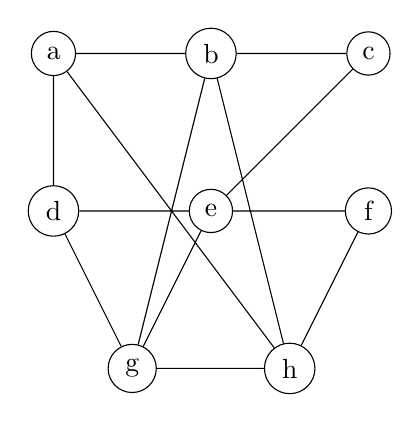
\begin{tikzpicture}
	\node[circle,draw](a) at (0,2) {a};
	\node[circle,draw](b) at (2,2) {b};
	\node[circle,draw](c) at (4,2) {c};
	\node[circle,draw](d) at (0,0) {d};
	\node[circle,draw](e) at (2,0) {e};
	\node[circle,draw](f) at (4,0) {f};
	\node[circle,draw](g) at (1,-2) {g};
	\node[circle,draw](h) at (3,-2) {h};

	\draw (a) -- (b) -- (c) -- (e) -- (d) -- (g) -- (h) -- (f) -- (e) -- (d) -- (a) -- (h) -- (b) -- (g) -- (e);
\end{tikzpicture}
\\
\\
1. Contract \( \left\{ a,d \right\}  \) \\

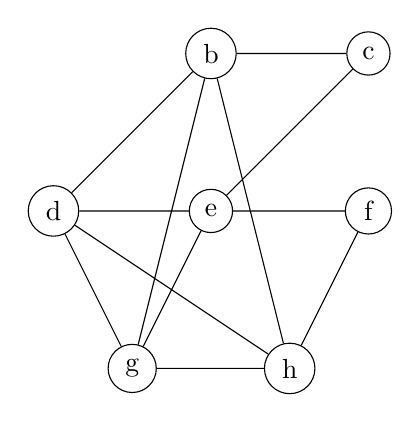
\begin{tikzpicture}
	\node[circle,draw](b) at (2,2) {b};
	\node[circle,draw](c) at (4,2) {c};
	\node[circle,draw](d) at (0,0) {d};
	\node[circle,draw](e) at (2,0) {e};
	\node[circle,draw](f) at (4,0) {f};
	\node[circle,draw](g) at (1,-2) {g};
	\node[circle,draw](h) at (3,-2) {h};

	\draw (d) -- (b) -- (c) -- (e) -- (d) -- (g) -- (h) -- (f) -- (e) -- (d) -- (h) -- (b) -- (g) -- (e);
\end{tikzpicture}
\\
\\
2. Contract \( \left\{ c,e \right\}  \) \\

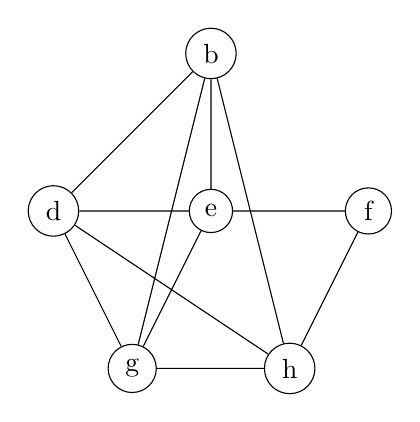
\begin{tikzpicture}
	\node[circle,draw](b) at (2,2) {b};
	\node[circle,draw](d) at (0,0) {d};
	\node[circle,draw](e) at (2,0) {e};
	\node[circle,draw](f) at (4,0) {f};
	\node[circle,draw](g) at (1,-2) {g};
	\node[circle,draw](h) at (3,-2) {h};

	\draw (d) -- (b) -- (e) -- (d) -- (g) -- (h) -- (f) -- (e) -- (d) -- (h) -- (b) -- (g) -- (e);
\end{tikzpicture}
\newpage
3. Contract \( \left\{ f,e \right\}  \) \\

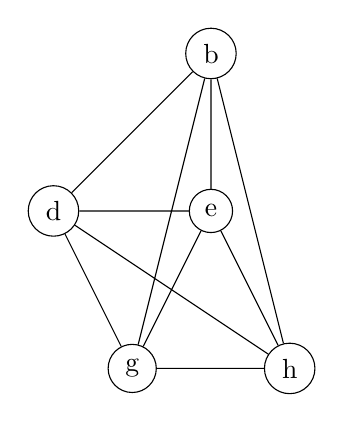
\begin{tikzpicture}
	\node[circle,draw](b) at (2,2) {b};
	\node[circle,draw](d) at (0,0) {d};
	\node[circle,draw](e) at (2,0) {e};
	\node[circle,draw](g) at (1,-2) {g};
	\node[circle,draw](h) at (3,-2) {h};

	\draw (d) -- (b) -- (e) -- (d) -- (g) -- (h) -- (e) -- (d) -- (h) -- (b) -- (g) -- (e);
\end{tikzpicture}

When we rearrange the nodes we can clearly see that it's a \( K_{5} \) graph. Thus \( G \) is not planar.\\
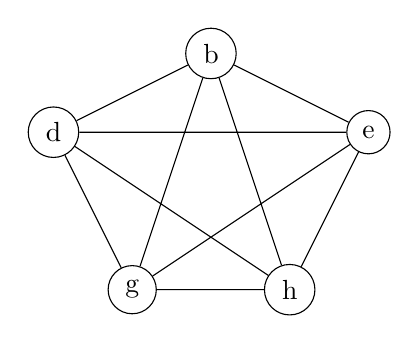
\begin{tikzpicture}
	\node[circle,draw](b) at (2,2) {b};
	\node[circle,draw](d) at (0,1) {d};
	\node[circle,draw](e) at (4,1) {e};
	\node[circle,draw](g) at (1,-1) {g};
	\node[circle,draw](h) at (3,-1) {h};

	\draw (d) -- (b) -- (e) -- (d) -- (g) -- (h) -- (e) -- (d) -- (h) -- (b) -- (g) -- (e);
\end{tikzpicture}
\section*{Exercise \homeworkNumber.2}

\begin{enumerate}[(a)]
	\item
	The syntactic interpretation is correct. \\
	Semantically what the natural language means to say is: Eat now or (eat later then food cold).
	Which would be: Eat Now $\lor($ eat later $\rightarrow$ food cold$)$.
	\item
	The syntactic interpretation is incorrect. What it expresses is Swimming $\rightarrow \neg$ Storm. \\
	That is also the semantic meaning.

\end{enumerate}



\section*{Exercise \homeworkNumber.3}

\begin{enumerate}[(a)]
	\item
	\( \mathcal I = \left\{ X \mapsto 0, Y \mapsto 1, Z \mapsto 0 \right\}  \).
	\item
	\begin{enumerate}[1)]
		\item $\mathcal I \models Y$
		\item $\mathcal I \not\models Z$
		\item $\mathcal I \models \neg Z$
		\item $\mathcal I \models Y \land \neg Z $ 
		\item $\mathcal I \models  \psi \lor (Y \land \neg Z)$ for all formulas $\psi$.
		\item $\mathcal I \not\models Y$
		\item $\mathcal I \models \neg Y$
		\item $\mathcal I \models \neg Y \lor \psi$ for all formulas $\psi$.
		\item From 5) and 8) we get $\mathcal I \models  (\psi \lor (Y \land \neg Z)) \land (\neg Y \lor \psi)$ for all formulas $\psi$. \\
		In particular $(X \lor (Y \land \neg Z)) \land (\neg Y \lor \neg X)$.
	\end{enumerate}
	\item 
	\( \mathcal I = \left\{ X \mapsto 0, Y \mapsto 0, Z \mapsto 0 \right\}  \).

\end{enumerate}



\section*{Exercise \homeworkNumber.4}

\begin{enumerate}[(a)]
	\item We will analyze the statement \( \phi = (((Y \land Z ) \to  X) \lor \lnot (X \lor  \lnot Z)) \)
	      over \( \left\{ X,Y,Z \right\}  \). \\
	      \textbf{Satisfiability}: Let \( \mathcal I = \left\{ X \mapsto 0, Y \mapsto 1, Z \mapsto 1 \right\}  \). We have \( \mathcal I \models X \) and \( \mathcal I \not\models Z \). From the definition of negation we have that \( \mathcal I \models \lnot Z \). Therefore, with the definition of disjuntion, we get \(  \mathcal I \not\models (X \lor \lnot Z ) \). With the definition of negation we have \(  \mathcal I \models \lnot (X \lor \lnot Z )\). With the definition of disjuntion we have \(  \mathcal I \models \psi \lor \lnot (X \lor \lnot Z )  \) for all formulas \( \psi \), in particular \( \mathcal I \models (((Y \land Z ) \to  X) \lor \lnot (X \lor  \lnot Z)) \). Therefore \( \phi \) is satisfiable. \\
	      \textbf{Falsifiability}:  The statement \( \phi \) is by the definition of disjuntion and negation false, iff both \(  ((Y \land Z ) \to  X)\) and \( \lnot(X \lor  \lnot Z) \) are false. The formula \( ((Y \land Z ) \to  X) \) is only false, if \( \mathcal I = \left\{ X \mapsto 0, Y \mapsto 1, Z \mapsto 1 \right\}  \). But under this interpretation, the formula \( \lnot(X \lor  \lnot Z) \) is true. Therefore \( \phi \) can never be false. \\
	      \textbf{Validness} The formula \( \phi \) is valid, since it can never be false. \\
	      \textbf{Unsatisfiability} The formula is not unsatisfiable because it's satisfiable.


	\item \( \phi = (A \land \lnot A) \land (B \land \lnot B) \)
\end{enumerate}



\end{document}
